\chapter{Auswertung}

Nach der Herstellung war bei einigen Proben mit blo�em Auge das Vorhandensein einer Gitterstruktur zu erkennen. Beim Betrachten der Proben unter einem bestimmten Winkeln war eine Begung des auftreffenden Lichts zu beobachten.

Die Betrachtung der hergestellten Gitterstrukturen unter dem Lichtmikroskop ist nicht n�tig, da die Aufl�sung zu gering ist um die Periodizit�t von ca 260~nm\todo{Stimmt das?} aufl�sen zu k�nnen (vgl. Abbildung \ref{fig:nix}). Zur Demonstration ist in Abbildung \ref{fig:400nm}\footnote[1]{Probe Hergestellt von Uwe Bog} ein Gitter  mit einer Periode von 400~nm unter 100-facher Vergr��erung dargestellt. Man erkennt deutlich die einzelnen Gitterlinien. Hier reicht das Lichtmikroskop gerade noch aus um die Strukturen aufzul�sen. 

\begin{figure}%
\centering
%\begin{adjustwidth}{0cm}{0cm}
	\subfloat[]{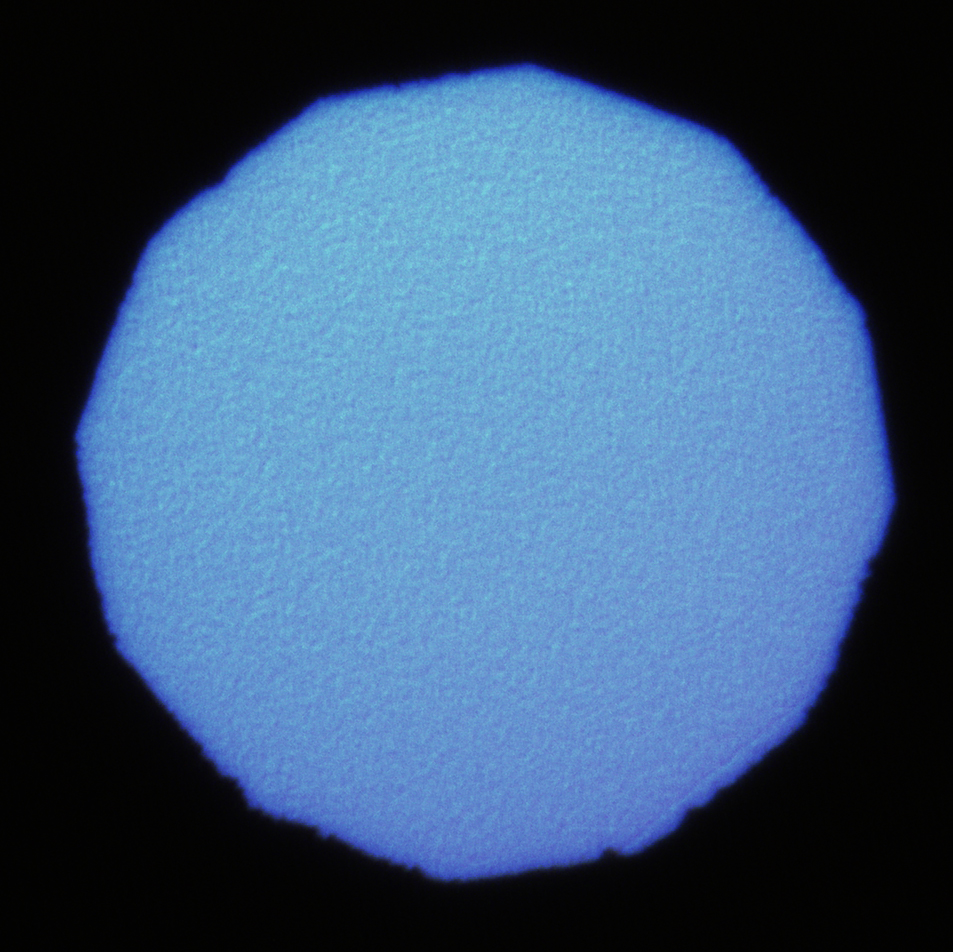
\includegraphics[totalheight=5 cm]{Grafiken/nix.jpg}\label{fig:nix}}\qquad
	\subfloat[]{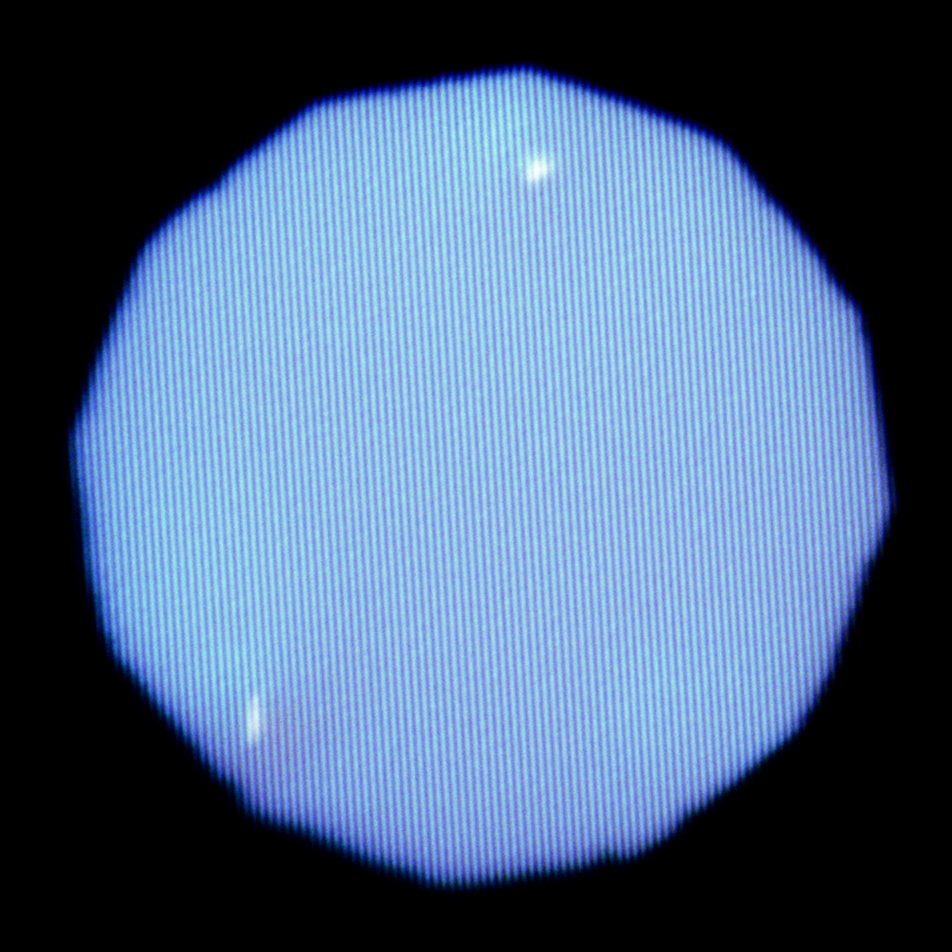
\includegraphics[totalheight=5 cm]{Grafiken/400nm.jpg} \label{fig:400nm}}\\%
%\end{adjustwidth}
\caption{Proben unter dem Lichtmikroskop. \textbf{(a)} Die Aufl�sung des Lichtmikroskops reicht nicht aus um die Strukturen aufzul�sen. \textbf{(b)} Gitterstruktur mit einer Periodizität von 400~nm.$^1$}%
\label{fig:matlab}%
\end{figure}



Um die hergestellten Proben zu Charakterisieren wurden die Proben am Institut f�r Mikrostrukturtechnik (IMT) mit einem \textit{Atomic Force Microscope} (AFM) vermessen. Abbildung \ref{fig:3d_bild} zeigt die mit dem AFM aufgezeichnete Topografie einer hergestellten Gitterstruktur.

\begin{figure}%
\centering
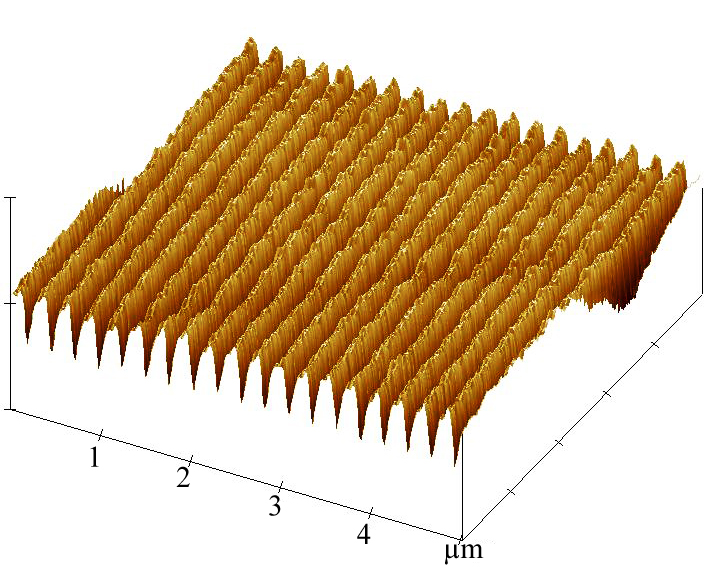
\includegraphics[width=.65\columnwidth]{Grafiken/3d_bild.jpg}%
\caption{AFM Messung der Topografie einer hergestellten Gitterstruktur (40~mJ, 4~s Entwicklungszeit).}%
\label{fig:3d_bild}%
\end{figure}



Im Folgenden sollen die Auswirkungen der Belichtungsdosis und der Entwicklungszeit auf die hergestellten Gitterstrukturen untersucht werden. Hierzu werden neben den im Rahmen des Laborversuches hergestellten Proben (vgl. Tabelle \ref{tab:parameter}) auch weitere Proben verwendet. Diese wurden im Labor Nanotechnologie von Matthias Ba�ler, Simon Jau� und Martin Waldvogel unter Anleitung von Uwe Bog hergestellt und vermessen.\footnote[2]{Ba�ler, Jau�, Waldvogel; Pr�sentation zum Laboversuch Laser Interverenz Lithographie; 15.08.2011} Tabelle \ref{tab:Referenz} zeigt die Herstellungsparameter dieser Proben.

\begin{table}%
\centering
\caption{Von Laborgruppe ''Ba�ler``$^2$ hergestellte Proben.}
\begin{tabular}{cc}

\toprule
Entwicklungsdauer	& Belichtungsenergien\\
in s	& in mJ\\
\midrule
10 & 10, 40, 80\\
20  & 10, 40, 80\\
30 & 10, 40, 80\\
\bottomrule 
\end{tabular}
\label{tab:Referenz}
\end{table}

